\documentclass[10pt]{article}
\usepackage[pdftex]{graphicx, color}
\usepackage{listings}
\usepackage{fancybox}
\usepackage{tikz}
\usepackage{multirow}
\usepackage{amsmath}
\usepackage{arydshln}
\usetikzlibrary{automata,positioning}

\headheight 8pt \headsep 20pt \footskip 30pt
\textheight 9in \textwidth 6.5in
\oddsidemargin 0in \evensidemargin 0in
\topmargin -.35in

\tikzset{
    state/.style={
           rectangle,
           rounded corners,
           draw=black, very thick,
           minimum height=2em,
           inner sep=2pt,
           text centered,
           },
}

\lstset{basicstyle=\small\ttfamily,breaklines=true}
\newcommand {\pts}[1]{{\bf #1 pts}}

\begin{document}
\begin{center}
\Large CS131 Compilers: Writing Assignment 2\\Due Sunday, April 15, 2018 at 23:29
\end{center}

\begin{center}
%% Change this:
\LARGE Rong Yuyang - 69850764
\end{center}

This assignment asks you to prepare written answers to questions on
context-free grammars and parsing. Each of the questions has a short answer. You
may discuss this assignment with other students and work on the problems
together. However, your write-up should be your own individual work.
and you should indicate in your submission who you worked with, if applicable. 
You should use the Latex template provided at the course web site to write your solution.

\begin{center}
%% Change this:
I worked with: (Name,ID), (Name,ID)...
\end{center}

\begin{enumerate}
  \item  \pts{$2\times 3= 6$} Give context-free grammar (CFG) for each of the following languages:
  \begin{enumerate}
           \item The set of all finite strings over the alphabet $\{0,1\}$ with an equal number of 0's and 1's.
            \[
            A \rightarrow 0A1A \mid 1A0A \mid \epsilon
            \]
           \item The set of all finite strings over the alphabet $\{0,1\}$ with the number of 0's greater than the number of 1's.
            \begin{equation*}\begin{aligned}
            & S \rightarrow Equal Zeros Equal \mid Equal Zeros Equal S \\
            & Equal \rightarrow 0Equal1Equal \mid 1Equal0Equal \mid \epsilon \\
            & Zeros \rightarrow 0 \mid 0Zeros \\
            \end{aligned}\end{equation*}
           \item The set $L_3=L_1\cap L_2$, where $L_1$ and $L_2$ are defined below.
           Let $L_1$ be the finite strings consisting of all non-empty \emph{palindromes} over the alphabet $\{a,b\}$. That is $L_1$
           consists of all sequences of a's and b's that read the same forward or backward. For example, $abba,~aabbbaa\in L_1$, but $abb\not\in L_1$.
           Let $L_2$ be the language over  $\{a,b\}$ representing the language of the regular expression $b(a+b)^\ast$.
            \begin{equation*}\begin{aligned}
            & S \rightarrow bPb \\
            & P \rightarrow aPa \mid bPb \mid \epsilon \\
            \end{aligned}\end{equation*}
  \end{enumerate}
  \newpage
  %
  \item \pts{$3\times 2= 6$} Consider the following CFG with terminals $\{(,),+,*,a,b\}$ ($+$ represents union) that is used to represent
regular expressions over alphabet $\{a, b\}$:
\[R\rightarrow R+R \mid RR\mid (R)\mid R^\ast \mid a\mid b\]
\begin{enumerate}
  \item Using the above CFG, provide a right-most derivation for the following input string $(a+(ba)^\ast b)^\ast$.
            \begin{equation*}\begin{aligned}
            R & \Rightarrow R^* \\
              & \Rightarrow (R)^* \\
              & \Rightarrow (R + R)^* \\
              & \Rightarrow (R + RR)^* \Rightarrow (R + Rb)^* \\
              & \Rightarrow (R + R^*b)^* \\
              & \Rightarrow (R + (R)^*b)^* \\
              & \Rightarrow (R + (RR)^*b)^* \\
              & \Rightarrow (R + (Ra)^*b)^* \Rightarrow (R + (ba)^*b)^* \Rightarrow (a + (ba)^*b)^* \\
            \end{aligned}\end{equation*}
  \item For the derivation in above solution, provide the corresponding parse tree.\\
	\begin{center}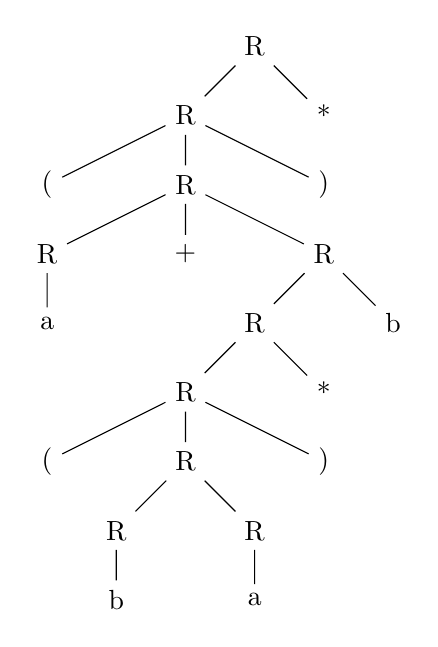
\begin{tikzpicture}[sibling distance=5em, level distance=2.5em]
		\node(root){R}
			child{node{R}
				child{node{(}}
				child{node{R}
					child{node{R}
						child{node{a}}}
					child{node{+}}
					child{node{R}
						child{node{R}
							child{node{R}
								child{node{(}}
								child{node{R}
									child{node{R}
										child{node{b}}}
									child{node{R}
										child{node{a}}}}
								child{node{)}}}
							child{node{*}}}
						child{node{b}}}}
				child{node{)}}}
			child{node{*}};
	\end{tikzpicture}\end{center}
\end{enumerate}



   \newpage

\item \pts{$3\times 3= 9$} Consider the following CFG.
\[\begin{array}{cll}
S & \rightarrow & AED \mid F \\
A & \rightarrow & Aa \mid a \\
B & \rightarrow & Bb \mid b \\
C & \rightarrow & Cc \mid c \\
D & \rightarrow & Dd \mid d \\
E & \rightarrow & bEc \mid bc \\
F & \rightarrow & aFd \mid BC
\end{array}\]

\begin{enumerate}
\item What is the language generated by this grammar?
            \begin{equation*}\begin{aligned}
            %% Your answer here
            \end{aligned}\end{equation*}
\item Is the grammar as given ambiguous? If yes, give an example of an expression
with two parse trees under this grammar. If not, explain why that is the case.\\\\
            $adbc$ is a good example with two parsing trees:
\begin{center}
\begin{tabular}{c|c}
            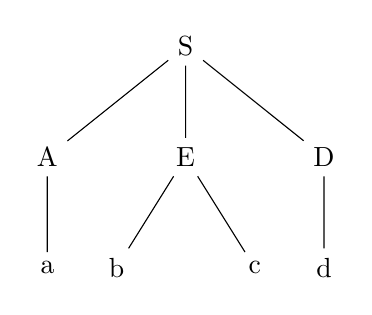
\begin{tikzpicture}[sibling distance=5em, level distance=4em]
            \node(root){S}
            	child{node{A}
            		child{node{a}}}
            	child{node{E}
            		child{node{b}}
            		child{node{c}}}
            	child{node{D}
            		child{node{d}}};
            \end{tikzpicture} 
            & 
            \begin{tikzpicture}[
            	level 1/.style={sibling distance=5em, level distance=2em},
            	level 2/.style={sibling distance=5em, level distance=2em},
            	level 3/.style={sibling distance=5em, level distance=2em},
            	level 4/.style={sibling distance=5em, level distance=2em},
            ]
            \node(root){S}
            	child{node{F}
            		child{node{a}}
            		child{node{F}
            			child{node{B}
            				child{node{b}}}
            			child{node{C}
            				child{node{c}}}}
            		child{node{d}}};
            \end{tikzpicture}
\end{tabular}
\end{center}
\item Transform the CFG given above by eliminating ambiguity and
left recursion, if needed.
            \begin{equation*}\begin{aligned}
            %% Your answer here
            \end{aligned}\end{equation*}
\end{enumerate}


   \newpage
\item \pts{$3\times 3= 9$} Consider the following CFG.
\[\begin{array}{cll}
A & \rightarrow & [AB] \mid a \\
B & \rightarrow & \epsilon \mid +AC \mid Cb \\
C & \rightarrow & \epsilon \mid -ABc
\end{array}\]

\begin{enumerate}
  \item Compute the First and Follow sets for the grammar.
            \begin{equation*}\begin{aligned}
            & FIRST([AB]) = \{[\} \\
            & FIRST(a) = a \\
            & FIRST(A) = FIRST([AB])\cup FIRST(a) = \{[, a\} \\
            & FIRST(\epsilon) = \{\epsilon\} \\
            & FIRST(-ABc) = \{-\}\\
            & FIRST(C) = FIRST(\epsilon) \cup FIRST(-ABc) = \{\epsilon, -\} \\
            & FIRST(+AC) = \{+\}\\
            & FIRST(Cb) = FIRST(C) = \{\epsilon, -\} \\
            & FIRST(B) = FIRST(\epsilon) \cup FIRST(+AC) \cup FIRST(Cb) = \{\epsilon, +, -, b\} \\
            & \\
            & FOLLOW(A) = \{+, -, b, c, \$\}\\
            & FOLLOW(B) = \{], c\} \\
            & FOLLOW(C) = \{], b, c\}
            \end{aligned}\end{equation*}
  \item Give the LL(1) parsing table for the grammar.\\
	\begin{table}[h]
	\centering
		\begin{tabular}{|c|c|c|c|c|c|c|c|c|}
		\hline
		\multirow{2}{*}{NT} & \multicolumn{8}{c|}{Input} \\ \cline{2-9} 
		                    &  [ & ] & a & + & - & b & c & $\$$\\ \hline
		A                   &  $A\rightarrow [AB]$ &   & $A\rightarrow a$ &   &   &   &   & \\ \hline
		\multirow{2}{*}{B}  &    & $B\rightarrow \epsilon$ &   & $B\rightarrow +AC$ & $B\rightarrow Cb$ & $B\rightarrow Cb$ & $B\rightarrow \epsilon$& \\ 
							&    & $B\rightarrow Cb$       & & & & & $B\rightarrow Cb$ & \\\hline
		C                   &    & $C\rightarrow \epsilon$ &   &   & $C\rightarrow -ABc$ & $C\rightarrow \epsilon$ & $C\rightarrow \epsilon$ & \\ \hline
		\end{tabular}
	\end{table}

  \item Is this grammar LL(1)? and Why. \\
  		No, it's not LL(1) due to two production rules' conflicts in the table.
\end{enumerate}
\newpage
\item \pts{$8$}  Using the context-free grammar for Cool given in Section 11 of the Cool
manual, draw a parse tree for the following expression.
  \begin{lstlisting}
    while not (x <-z <- 0) loop
      y <- z + 2 * x + 1
    pool
  \end{lstlisting}
Note that the context-free grammar by itself is ambiguous, so you will
need to use the precedence and associativity rules in Section 11.1 to
get the correct tree. \\
        \begin{center}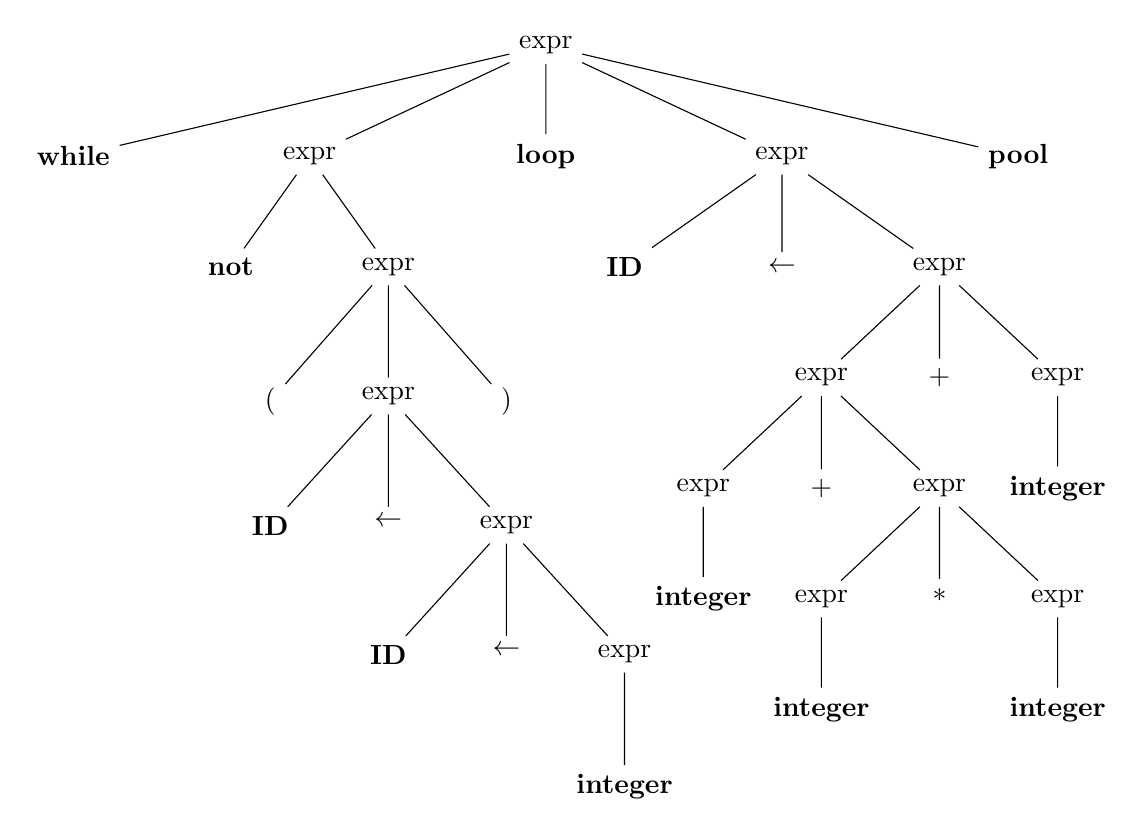
\begin{tikzpicture}    [
        level distance = 4em,
	    level 1/.style={sibling distance=3cm},
	    level 2/.style={sibling distance=2cm},
	    level 3/.style={sibling distance=1.5cm},
	    level 4/.style={sibling distance=1.5cm},
	    level 5/.style={sibling distance=1.5cm},
	    level 6/.style={sibling distance=1.5cm},
    	]
        \node(root){expr}
        	child{node{\textbf{while}}}
        	child{node{expr}
        		child{node{\textbf{not}}}
        		child{node{expr}[below]
        			child{node{(}}
        			child{node{expr}
        				child{node{\textbf{ID}}}
        				child{node{$\leftarrow$}}
        				child{node{expr}
        					child{node{\textbf{ID}}}
        					child{node{$\leftarrow$}}
        					child{node{expr}
        						child{node{\textbf{integer}}}
        					}
        				}
        			}
        			child{node{)}}
        		}
        	}
        	child{node{\textbf{loop}}}
        	child{node{expr}
        		child{node{\textbf{ID}}}
				child{node{$\leftarrow$}}
				child{node{expr}
					child{node{expr}
						child{node{expr}
							child{node{\textbf{integer}}}}
						child{node{+}}
						child{node{expr}
							child{node{expr}
								child{node{\textbf{integer}}}
							}
							child{node{*}}
							child{node{expr}
								child{node{\textbf{integer}}}
							}
						}
					}
					child{node{+}}
					child{node{expr}
						child{node{\textbf{integer}}}
					}
				}
        	}
        	child{node{\textbf{pool}}};

        \end{tikzpicture}\end{center}

\newpage
\item \pts{$4\times 4 =16$} Consider the following grammar describing a certain sort of nested lists:
\[\begin{array}{cll}
S & \rightarrow & T;S \mid \epsilon \\
T & \rightarrow & U\star T \mid U \\
U & \rightarrow & x\mid y\mid [S]
\end{array}\]
$S$, $T$, and $U$ are nonterminals, while others are terminals.
\begin{enumerate}
  \item Left-factor this grammar.
		\[\begin{array}{cll}
		S & \rightarrow & T;S \mid \epsilon \\
		T & \rightarrow & UT'  \\
		T' & \rightarrow & \star T \mid \epsilon\\
		U & \rightarrow & x\mid y\mid [S]
		\end{array}\]
  \item Give the First and Follow sets for each nonterminal in the grammar obtained in part (a).
            \begin{equation*}\begin{aligned}
			& FIRST(S) = \{x, y, [, \epsilon\} \\
			& FIRST(T) = \{x, y, [\} \\
			& FIRST(T') = \{\star, \epsilon\} \\
			& FIRST(U) = \{x, y, [\} \\
			& \\
			& FOLLOW(S) = \{\$, ]\} \\
			& FOLLOW(T) = \{;\} \\
			& FOLLOW(T') = \{;\} \\
			& FOLLOW(U) = \{;, \star\} \\
            \end{aligned}\end{equation*}
  \item Using this information, construct an LL(1) parsing table for the grammar obtained in part (a).

	\begin{table}[h]
		\centering
		\caption{My caption}
		\label{my-label}
		\begin{tabular}{|c|c|c|c|c|c|c|c|}
		\hline
		\multirow{2}{*}{NT} & \multicolumn{7}{c|}{Input} \\ \cline{2-8} 
		                    & [ & ] & x & y & ; & $\star$ & \$  \\ \hline
		S                   & $S \rightarrow T;S$ & $S \rightarrow \epsilon$ & $S \rightarrow T;S$ & $S \rightarrow T;S$ &  &  & $S \rightarrow \epsilon$  \\ \hline
		T                   & $T \rightarrow UT'$ &  & $T \rightarrow UT'$ & $T \rightarrow UT'$ &  &  &  \\ \hline
		T'                  &  &  &  &  & $T' \rightarrow \epsilon$ & $T' \rightarrow \star T$ &  \\ \hline
		U                   & $U\rightarrow[S]$ &  & $U\rightarrow x$ & $U\rightarrow y$ &  &  &  \\ \hline
		\end{tabular}
	\end{table}

  \item Suppose we generated an LL(1) parser for the grammar using the table you constructed. What would go wrong if it tried to parse the following input string?
  \[[x;y]\star [;\] \\
  		It will raise an error when encountered the last semi-colon, as it is in state $S$ and a semi-colon(;) is an illegal input.
\end{enumerate}

\newpage
\item \pts{$3\times 2+5\times 2 =16$} Consider the following CFG, which has the set of terminals
$T = \{ \textbf{a}, \textbf{b} \}$.
\[\begin{array}{cll}
 S & \rightarrow & X \textbf{a} \\
X & \rightarrow & \textbf{a} \mid \textbf{a} X \textbf{b}
\end{array}\]

\begin{enumerate}

\item Construct a DFA for viable prefixes of this grammar using LR(0)
items.
	\begin{center}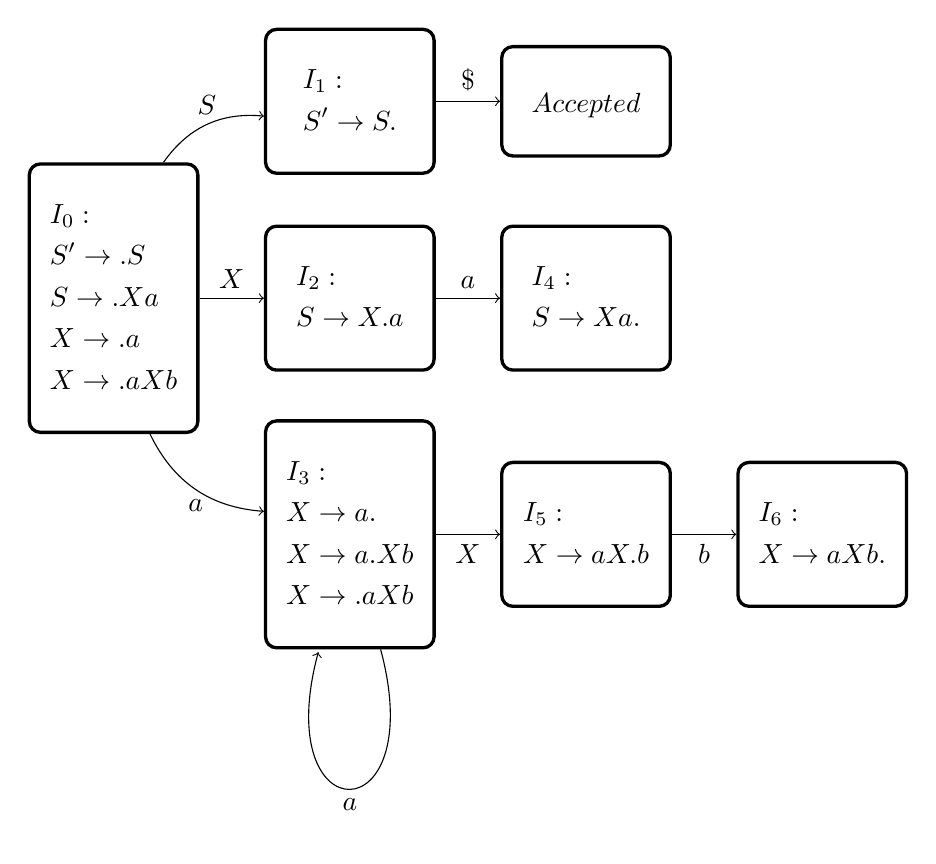
\begin{tikzpicture}
		\node[state] (I0) { 
			\parbox{2cm}{\begin{equation*}\begin{aligned}
				& I_0: \\
				& S' \rightarrow .S \\
				& S\rightarrow .Xa \\
				& X\rightarrow .a \\
				& X\rightarrow .aXb \\
			\end{aligned}\end{equation*}}
		};

		\node[state, right of=I0, node distance=3cm] (I2){
			\parbox{2cm}{\begin{equation*}\begin{aligned}
				& I_2: \\
				& S\rightarrow X.a \\
			\end{aligned}\end{equation*}}
		};		
		\node[state, above of=I2, node distance=2.5cm] (I1) { 
			\parbox{2cm}{\begin{equation*}\begin{aligned}
				& I_1: \\
				& S' \rightarrow S. \\
			\end{aligned}\end{equation*}}
		};

		\node[state, right of=I1, node distance=3cm] (acc){
			\parbox{2cm}{\begin{equation*}\begin{aligned}
				& Accepted \\
			\end{aligned}\end{equation*}}
		};
		\node[state, right of=I2, node distance=3cm] (I4){
			\parbox{2cm}{\begin{equation*}\begin{aligned}
				& I_4: \\
				& S\rightarrow Xa. \\
			\end{aligned}\end{equation*}}
		};
		\node[state, below of=I2, node distance=3cm] (I3){
			\parbox{2cm}{\begin{equation*}\begin{aligned}
				& I_3: \\
				& X\rightarrow a. \\
				& X\rightarrow a.Xb \\
				& X\rightarrow .aXb \\
			\end{aligned}\end{equation*}}
		};
		\node[state, right of=I3, node distance=3cm] (I5){
			\parbox{2cm}{\begin{equation*}\begin{aligned}
				& I_5: \\
				& X\rightarrow aX.b \\
			\end{aligned}\end{equation*}}
		};
		\node[state, right of=I5, node distance=3cm] (I6){
			\parbox{2cm}{\begin{equation*}\begin{aligned}
				& I_6: \\
				& X\rightarrow aXb. \\
			\end{aligned}\end{equation*}}
		};
		\path[->]
		(I0) 	edge 					node[above]{$X$} (I2)
				edge 	[bend right] 	node[below]{$a$} (I3)
				edge 	[bend left] 	node[above]{$S$} (I1)
		(I1) 	edge 				 	node[above]{$\$$} (acc)
		(I2) 	edge 					node[above]{$a$} (I4)
		(I3) 	edge 	[loop below] 	node[below]{$a$} ()
				edge 					node[below]{$X$} (I5)
		(I5) 	edge 					node[below]{$b$} (I6);
		
	\end{tikzpicture}\end{center}
\item Identify a shift-reduce conflict in this grammar under the
SLR(1) rules.\\ 
	\begin{equation*}\begin{aligned}
		& 1: S\rightarrow Xa  \\
		& 2: X\rightarrow a \\		
		& 3: X\rightarrow aXb \\
	\end{aligned}\end{equation*}
	\begin{table}[h]
	\centering
	\begin{tabular}{c|ccc|cc}
		\hline
		\multirow{2}{*}{State} & \multicolumn{3}{c|}{Actions} & \multicolumn{2}{c}{Goto} \\ \cline{2-6} 
		                  &  $a$  &  $b$  &  $\$$ &    $S$    &    $X$    \\ \hline
		       0          &   s3  &       &       &     s1    &     s2    \\
		       1          &       &       &  acc  &           &           \\
		       2          &   s4  &       &       &           &           \\
		       3          & \textbf{s3/r2} &   r2  &       &           &     s5    \\
		       4          &       &       &   r1  &           &           \\
		       5          &       &   s6  &       &           &           \\
		       6          &   r3  &   r3  &       &           &           \\ \hline	
	\end{tabular}
	\end{table}
	\\
	There is one in $I_3$ where the parser have to decide whether to reduce
	$X\rightarrow a.$ or keep shifting if there is $X$ or $a$ incoming.
	\\
\item Assuming that an SLR(1) parser resolves shift-reduce conflicts
by choosing to shift, show the operation of such a parser on the input
string \textbf{aaba}.
	\\
	\begin{table}[h]
	\begin{center}\begin{tabular}{l|r|l}
	\textbf{Stack} & \textbf{Input} & \textbf{Action} \\ 
	\$ & aaba\$ & shift \\ 
	\$a & aba\$ & shift \\ 
	\$aa & ba\$ & reduce by $X\rightarrow a$ \\ 
	\$aX & ba\$ & shift \\ 
	\$aXb & a\$ & reduce by $X\rightarrow aXb$ \\ 
	\$X & a\$ & shift\\
	\$Xa & \$ & reduce by $S\rightarrow Xa$ \\ 
	\$S & \$ &  $Accepted$\\ 
	\end{tabular}\end{center}
%	\end{table}
%	\begin{table}[h]
%	\begin{center}\begin{tabular}{l|r|l}
%	\textbf{Stack} & \textbf{Input} & \textbf{Action} \\ 
%	\$ & aaba\$ & shift \\ 
%	\$a & aba\$ & shift \\ 
%	\$aa & ba\$ & error \\ 
%	\end{tabular}\end{center}
	\end{table}
	\\
\item Suppose that the production $X \rightarrow \varepsilon$ is added
to this grammar.  Identify a reduce-reduce conflict in the resulting
grammar under the SLR(1) rules.
          \[
            %% Your answer here
            \]
\end{enumerate}
\end{enumerate}
\end{document}

